\chapter{Time Series: Clustering and Classification}

\section{Clustering}

For time series, the most common methods are Partitional Clustering and Hierarchical Clustering. \textbf{Partitional Clustering} uses the K-means algorithm (or some variant) to optimize the objective function by minimizing the SSE. \textbf{Hierarchical Clustering} starts by computing pairwise distance between time series (using whatever appropriate distance measure is specified by the user), and then merges clusters in a bottom-up way, merging at each step the two closest clusters, until the cluster containing all data points is obtained. This approach is however limited to small datasets, since it is computationally complex.

Time series clustering can be of the following types:
\begin{itemize}
    \item \textbf{Whole clustering}: the conventional type of clustering, where the goal is to assign each data object to a cluster.

    \item \textbf{Feature-based clustering}: features (or motifs, see next section) are extracted from the series, and then used to cluster.

    \item \textbf{Compression-based clustering}: compress time series and run clustering on the compressed versions.

    \item \textbf{Subsequence clustering}: subsequence clustering is done on the subsequences extracted from a single long time series using a sliding window.
\end{itemize}

\section{Motif and Discord Discovery}

\textbf{Motifs} are repeated patterns within a time series. \textbf{Discords} are exceptionally unusual patterns withing a time series. Motif discovery is a preprocessing phase for other analysis: mining association rules, where motifs are referred to as primitive shapes and frequent patterns, classification, which in some cases works by constructing typical prototypes (motifs) of each class, and anomaly detection, in which algorithms use motifs to model typical time series behaviour and detect future patterns that are dissimilar.

Given a predefined motif length $m$, a brute-force approach would simply search all possible motifs obtainable from all possible comparisons of subsequences of length $m$. This approach is clearly inefficient; the most commonly used algorithm was originally developed in bioinformatics, and is based on \textbf{random projections} and SAX.

First, an alphabet size $\alpha$, SAX window size $w$, and motif length $n$ are set. All approximated subsequences of length $w$ are extracted via SAX from the time series by shifting forward the window one measurement at a time, for a total of $|T| - (n - 1)$ subsequences. Then, a mask is randomly chosen to only select certain ``columns'' of the subsequences; i.e., if the mask $\{1,3\}$ is chosen, only the first and third symbols in the representation are considered. Collisions between masked subsequences are recorded with a \textbf{collision matrix}, increasing the value in the corresponding cell. This step is repeated multiple times choosing different masks.

At the end of these random perturbations, motifs can be observed in the collision matrix, looking at the cells that have the highest values: their indexes are the positions in which the motifs start in the time series. The problem with this approach, however, is that it is highly dependent on the approximation technique used.

\subsection{Matrix Profile}

Given a time series $T$, and having calculated the pairwise distance among all the $|T| - (n - 1)$ subsequences that can be extracted from $T$ using a sliding window of length $n$, the \textbf{Matrix Profile} (\textbf{MP}) of a $T$ is the vector that annotates the distance between each subsequence and its nearest neighbor. The index of the corresponding nearest neighbor of each subsequence is stored in a vector called \textbf{Matrix Profile Index}, which can be used to find the nearest neighbor in constant time. Pointers are not necessarily symmetric: if $n$ is the nearest neighbor of $m$, the nearest neighbor of $n$ is not necessarily $m$, but may be some other subsequence. However, for the two smallest values in the MP, the pointers of the corresponding subsequences must be mutual.

\begin{figure}[h]
    \centering
    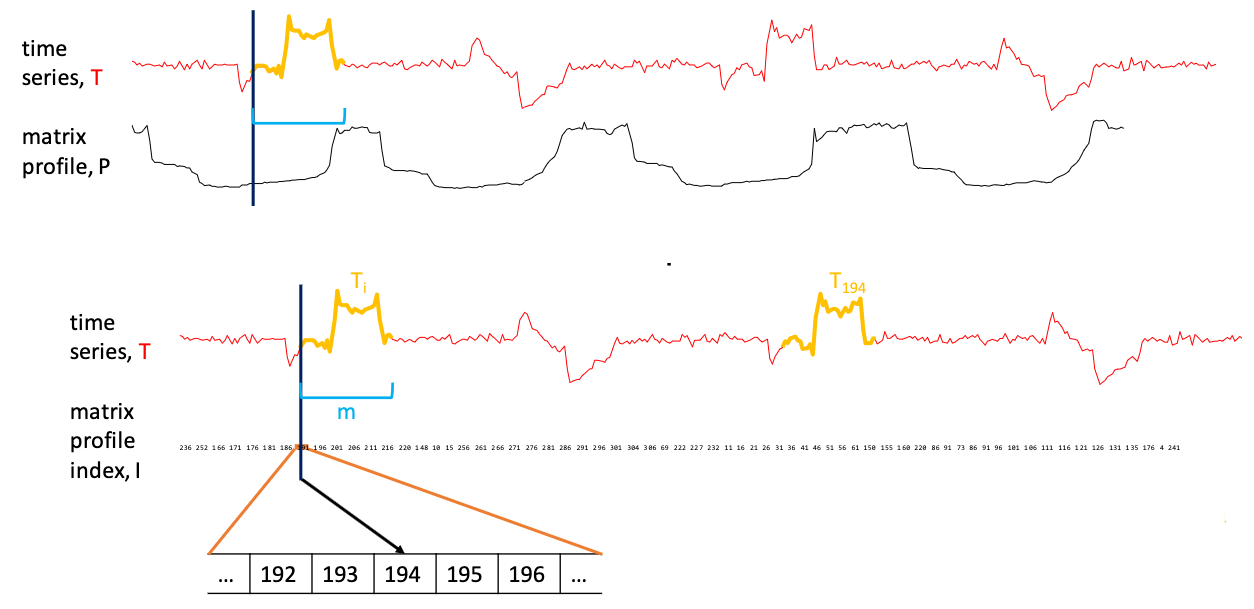
\includegraphics[width=0.9\linewidth]{img/mp_mpi.png}
    \caption{Matrix Profile (on top) and Matrix Profile Index (on the bottom).}
    \label{fig:mp-mpi}
\end{figure}

Low values in the matrix profile indicate that the corresponding subsequence has at least one similar subsequence in the data: these regions indicate motifs. Areas that instead have very high values indicate discords, since they are subsequences whose nearest neighbor is very distant.

To compute the matrix profile of a time series, the cells of the vector are initialized to $\infty$. Then, a random subsequence $T_i$ is selected, and the distance with every other subsequence is stored in a different vector. This step has complexity $O(|T| \log(|T|))$. The matrix profile is updated, applying element-wise minimum to the two vectors (skipping the cell for $T_i$). A new subsequence is randomly selected, and the process is repeated, updating the matrix profile with the new minimum values. The algorithm stops once all subsequences have been selected. The total time complexity is $O(|T|^2 \log(|T|))$.

It may be useful to think of time series subsequences as points in an $m$ dimensional space: subsequences that are very similar will be close together in denser areas, which will in turn correspond to regions in the MP with low values. To understand how the top-k motifs are extracted, we can consider this data-point interpretation. A parameter $R > 1$ is chosen, and the two nearest points are found, called the \textbf{motif pair}. Given the distance $D_1$ between these two points, a circle with radius $D_1 * R$ is drawn around each point: any point that falls within either circles are added to this motif: this is the top-1 motif. To find the top-2 motif, the next closest pair of points is found (excluding the ones in the previous motif), whose distance is $D_2 > D_1$. Again, a circle of radius $D_2 * R$ is drawn around each circle, and all points in this circle are added to the motif. To choose when to stop, i.e., to choose the value of $k$, we can either use a predefined value, or use the Minimum Description Length.

\begin{figure}[h]
    \centering
    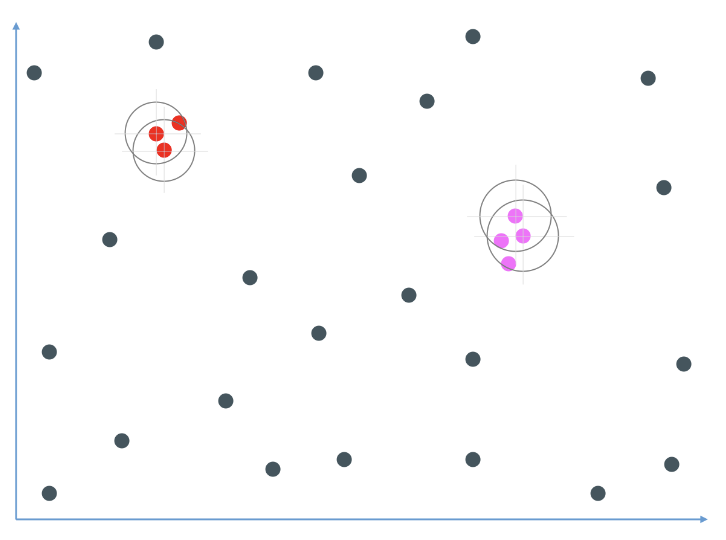
\includegraphics[width=0.5\linewidth]{img/topk_motifs.png}
    \caption{A graphical interpretation of how top k-motifs are found. The red dots are the top 1-motif, and the magenta ones are the top-2 motifs.}
    \label{fig:top-k-motifs}
\end{figure}

If we're interested in finding top-k discords instead, a parameter $E$ is set to select how many subsequences will be excluded in the vicinity of the anomaly, and the subsequence with the highest distance in the MP is found. The $E$ closest subsequences to the anomaly are selected, and removed with the anomaly. Again, the value of $k$ can be either set to a predefined value or chosen as the MDL.

\section{Classification}

For classification tasks, given a set of $n$ time series all assumed of length $m$, each time series $x_i$ is associated with a class label $c_i$. The objective is to find a target function $f$ that maps all possible time series to the space of possible class labels. The most widely used algorithm for time series classification is K-NN, used in the raw data. It is simple, and can be used with Dynamic Time Warping. However, it is a lazy classifier, meaning that prediction is costly as it is, and DTW slows the execution even further. Additionally, K-NN based classification does not provide much insight into the data.

An alternative is shapelet-based classification. \textbf{Shapelets} are time series subsequences that are maximally representative of a class. Once extracted, shapelets can be used to transform the dataset so that it can be used as input for classifiers; additionally, they provide interpretable results, and can be incredibly accurate since they are local features, unlike most other time series classifiers which only consider global features. They also tend to be faster at classification compared to other methods, since the time complexity of the prediction phase is only $O(ml)$, where $m$ is the length of the query time series, and $l$ is the length of the shapelet. In contrast, DTW-based K-NN has a time complexity of $O(km^3)$, where $k$ is the number of objects in the training set.

Since shapelets are much shorter than the time series they're extracted from, we need to define a measure to evaluate the similarity between a subsequence and a time series. The distance between two time series $T$ and $S$, with $|S| < |T|$, is calculated via:
\begin{equation*}
    \textit{SubsequenceDist}(T,S) = \min(\textit{Dist}(S,S')) \ \forall S' \in S_T^{|S|}
\end{equation*}
where $S_T^{|S|}$ is the set of all possible subsequences of $T$. This function returns the distance between $S$ and the ``best matching'' location in $T$. Each time series in a dataset can be represented as a vector of distances with the shapelets extracted from them: if a given time series belongs to a certain class, it will be very close to the representative shapelet(s) of that specific class, and further away from shapelets that represent other classes.

\begin{figure}[h]
    \centering
    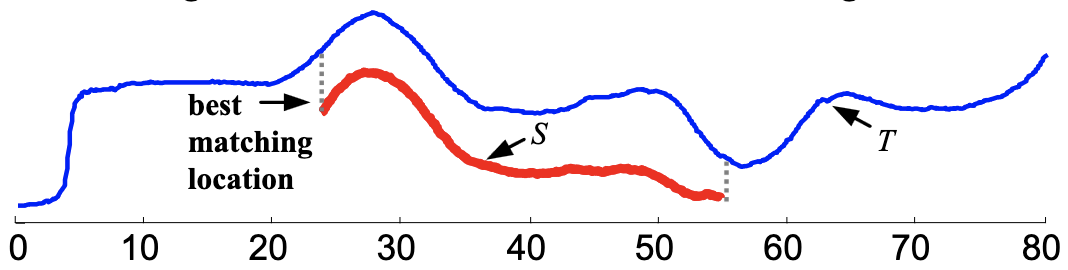
\includegraphics[width=0.5\linewidth]{img/subsequencedist.png}
    \caption{The best matching location of $S$ over $T$.}
    \label{fig:subseq-dist}
\end{figure}

\subsection{Shapelet Extraction}

The simplest way to extract shapelets is the brute-force approach, which generates all possible subsequences of all possible lengths from the time series in the dataset, adding them to the pool of candidates. Assume the time series are each assigned to one of two possible class labels. For each candidate, the algorithm must check how well it separates the objects of one class from the other, and choose the candidate that performs best. First, all time series are rearranged in the dataset based on the distance from the current candidate; then, the optimal split point that maximizes the \textbf{information gain} is found, similarly to how splits are chosen in Decision Tree training algorithms. After calculating the information gain of all candidates, the one with the highest value is selected.

A common measure used to evaluate information gain is entropy:
\begin{equation*}
    I(D) = -p(A) \log_2 (p(A)) -p(B) \log_2 (p(B)) \,,
\end{equation*}
where $p(A)$ and $p(B)$ are the proportion of objects belonging to each respective class $A$ and $B$. Given a strategy that divided the dataset $D$ into two subsets $D_1$ and $D_2$, the information remaining in the dataset after the split is calculated as the weighted average entropy of each subset.
If the fraction of objects in $D_1$ is $f(D_1)$, and the fraction of objects in $D_2$ is $f(D_2)$, the total entropy of the dataset after a split is calculated as:
\begin{equation*}
    \hat{I}(D) = f(D_1)I(D_1) + f(D_2)I(D_2)
\end{equation*}
The information gain for a splitting rule is given by the difference of the entropy before and after the split:
\begin{equation*}
    \textit{Gain}(\textit{split}) = I(D) - \hat{I}(D)
\end{equation*}

The total number of candidates generated by the brute-force approach amounts to:
\begin{equation*}
    \sum_{l = \textit{minlen}}^{\textit{maxlen}} \sum_{T_i \in D}(|T_i| - l + 1)
\end{equation*}
Then, for each of these candidates, the distance with every training time series must be calculated, as well as the entropy for each split. Obviously, this solution is highly space and time inefficient; two speedup methods are:
\begin{itemize}
    \item \textbf{Distance Early Abandon}: in the brute-force approach, the distance from the time series $T$ with the subsequence $S$ is done by calculating the Euclidean distance between each subsequence of length $|S|$ in $T$ and $S$, and choosing the minimum. This operation costs $O(|T|)$. However, the only distance we need is the one we keep, i.e., the minimum one. Instead of calculating all distances, the calculations can stop after the distance starts to increase compared to the smallest value recorded so far; this technique is known as early abandon.

    \item \textbf{Admissible Entropy Pruning}: we want to find only the best shapelet for each class. Obtaining the distance between a candidate and its nearest matching subsequence in each time series in the dataset is the most expensive operation. Instead of waiting until all distances from all time series are calculated, an upper bound of the information gain can be calculated based on the distances known so far. If at any point this upper bound cannot beat the best-so-far information gain, the distance calculations are stopped, pruning the candidate, since there's no way it could ever be better than the best candidate found so far. This is done by comparing the information gain of the best candidate with the information gain of the current one where all training instances that haven't been compared yet are assumed to be perfectly classified. 
\end{itemize}



